\documentclass[12pt]{article}%
\usepackage{amsfonts}
\usepackage{fancyhdr}
\usepackage{comment}
\usepackage[a4paper, top=2.5cm, bottom=2.5cm, left=2.2cm, right=2.2cm]%
{geometry}
\usepackage{times}
\usepackage{graphicx}

\usepackage{hyperref}

\usepackage{amssymb}
\usepackage{graphicx}%

\begin{document}

\title{MLT - Assignment 2}
\author{Ayush Sekhari}
\date{\today}
\maketitle

\section{Observations}
\begin{enumerate}
\item We do not have missing attributes
\end{enumerate}

\section{Part-a}
I performed a binary search between 2 and 450 and chose the point at which the data started to level off. That is, the error is in the difference range of 4.5\%-5\% of the minimum error.  

The number of trees where the error curve started to level off:  198 and error at this point is : 3.515\%

The plot is shown in the figure below and the levelling off point has been marked in red.

\begin{figure}
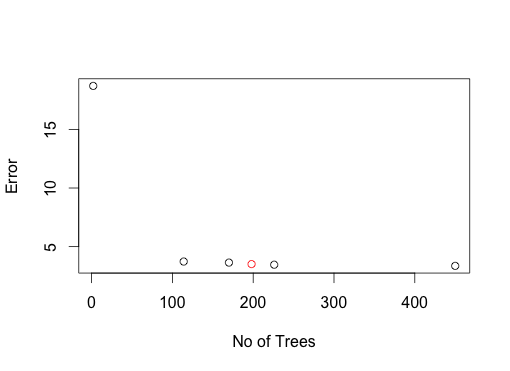
\includegraphics{part.png}
\caption{Plot of error rates vs number of trees while performing Binary search}
\end{figure}

\begin{figure}
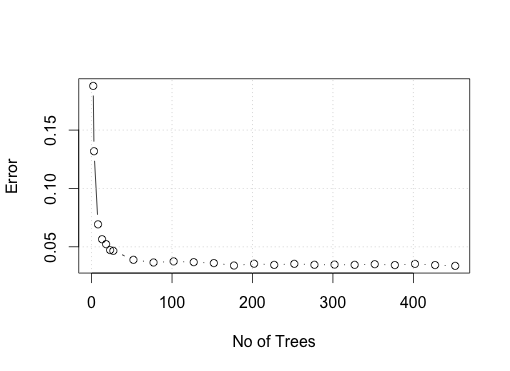
\includegraphics{part1.png}
\caption{General Trend of Error vs Number of Trees for Random Forest}
\end{figure}


\section{Part-b}
The tree size for the above case = 198, The OOB error for this forest over the entire training data is = 3.195\%

\section{Part-c}

The data table shows that too much randomness or strictness is not good. I get comparatively higher error for small values of m(i.e. m = 1 , more randomness) and for large values of m(i.e. m = 8 , less randomness).


\begin{table}[!h]
\begin{center}

\begin{tabular}{|c|c|}
\hline
{\bf m Value} & {\bf  CV error }\\ \hline
 {\bf m = 1 } &  0.05145\\ \hline
 {\bf m = 2 } &  0.03450\\ \hline
 {\bf m = 3 } &  0.03465\\ \hline
 {\bf m = 4 } &  0.03510\\ \hline
 {\bf m = 5 } &  0.03625\\ \hline
 {\bf m = 6 } &  0.03685\\ \hline
 {\bf m = 7 } &  0.03800\\ \hline
 {\bf m = 8 } &  0.04105\\ \hline

\end{tabular}

\caption{CV errors for different values of splitting attribute number for trees in the forest}
\end{center}
\end{table}

\section{Part-d}
In this part, I used the same algorithm as in Part - (a) to find the point where the error curve levels off.
\begin{itemize}
\item Figures 3 and 4 show the plot of  5 fold cross-validated error for a forest with T trees against the size of the sampled data set expressed as a percentage of L when 4 attributes are randomly used for splitting. It has a local minima at 60\% with error value = 3.745\%.
\item Figures 5 and 5 show the plot of  5 fold cross-validated error for a forest with T trees against the size of the sampled data set expressed as a percentage of L when all the  attributes are used for splitting. It has a local minima at 55\% with error value = 5.64\%.
\item This shows that the maximum accuracy comes when training data is $\sim$ 55-60\% of the total data available for training.
\item High values of the error for the cases of smaller sample sizes is because we do not have much data to train on, therefore the random forest formed has lesser strength and correspondingly lesser accuracy. 
\item We observe high error values when sample size is large because there would be a huge sharing of training data between the two trees. This increases the correlation in the forest and thus the accuracy decreases.
\item  In case of bagging, the expected size of the bag is $\sim$ 63\% of the training data available.
\item  Since, most accuracy comes at around $\sim$55-60\%, this shows that bagging is a good approximation for fixing training data for trees in the forest. 
\item I would prefer bagging as it introduces randomness in the model. There may be some trees trained on bigger data sets and some trained on smaller data sets. This introduces variation in the forest which is good to some amount. 
\item With bagging we get an error of 5.665\% with 52 trees which is comparable to the minimum error observed with no bagging. 

\end{itemize}

\begin{figure}
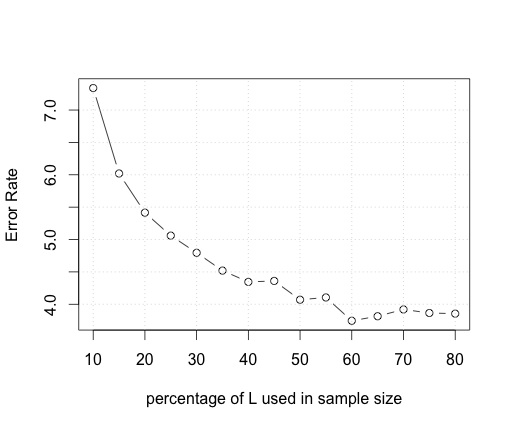
\includegraphics{part4.png}
\caption{5 fold cross-validated error for a forest with T trees against the size of the sampled data set expressed as a percentage of L with mtry = 4}
\end{figure}

\begin{figure}
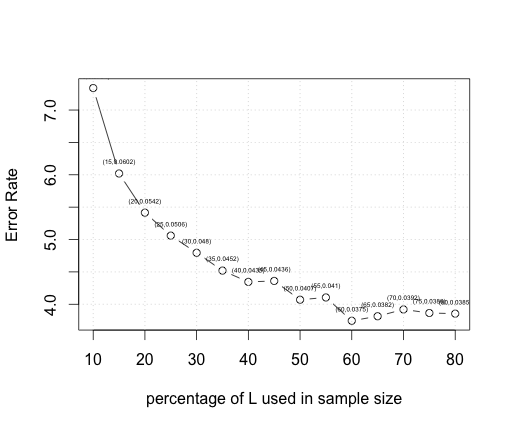
\includegraphics{part41.png}
\caption{5 fold cross-validated error for a forest with T trees against the size of the sampled data set expressed as a percentage of L with mtry = 4}
\end{figure}

\begin{figure}
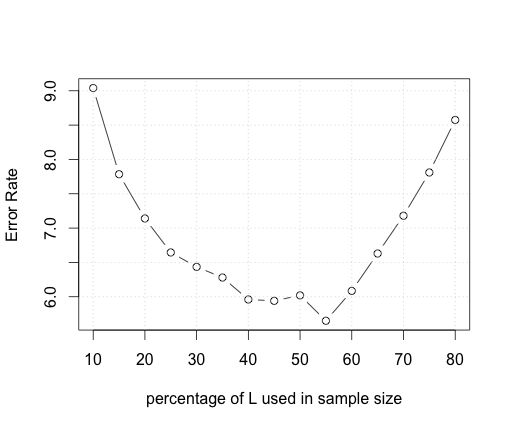
\includegraphics{part4a.png}
\caption{5 fold cross-validated error for a forest with T trees against the size of the sampled data set expressed as a percentage of L with mtry = 16}
\end{figure}

\begin{figure}
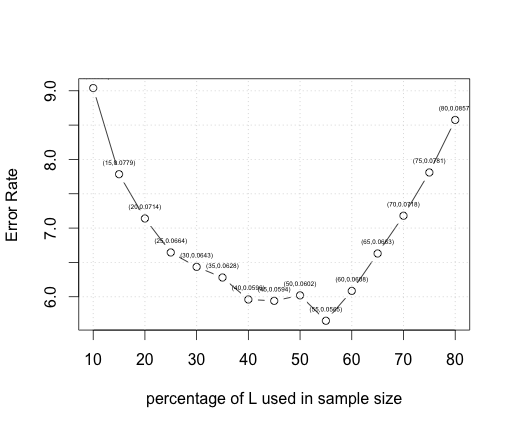
\includegraphics{part41a.png}
\caption{5 fold cross-validated error for a forest with T trees against the size of the sampled data set expressed as a percentage of L with mtry = 16}
\end{figure}


\end{document}
